\documentclass[conference]{IEEEtran}
\IEEEoverridecommandlockouts
% IEEE conference template, version as of 6/27/2024

\usepackage{cite}
\usepackage{amsmath,amssymb,amsfonts}
\usepackage{algorithmic}
\usepackage{graphicx}
\usepackage{textcomp}
\usepackage{xcolor}
\usepackage{url}
\usepackage{iftex}
\ifXeTeX
  % XeTeX (e.g. Tectonic): Times-compatible text and maths, as IEEEtran gives under pdfLaTeX
  \usepackage{fontspec}
  \setmainfont{texgyretermes}[Extension=.otf, UprightFont=*-regular, BoldFont=*-bold, ItalicFont=*-italic, BoldItalicFont=*-bolditalic]
  \usepackage{unicode-math}
  \setmathfont{texgyretermes-math.otf}
\fi
\def\BibTeX{{\rm B\kern-.05em{\sc i\kern-.025em b}\kern-.08em
    T\kern-.1667em\lower.7ex\hbox{E}\kern-.125emX}}
\begin{document}

\title{Strata Cobot: Autonomous Ore Sorting and Haulage with a Manipulator and a Mobile Robot in ROS~2}

\author{\IEEEauthorblockN{C Saihardhik Reddy}
\IEEEauthorblockA{\textit{Amrita Vishwa Vidyapeetham}\\
India}
\and
\IEEEauthorblockN{R Gagan Chowdary}
\IEEEauthorblockA{\textit{Amrita Vishwa Vidyapeetham}\\
India}
\and
\IEEEauthorblockN{K Charan Saatvikh Reddy}
\IEEEauthorblockA{\textit{Amrita Vishwa Vidyapeetham}\\
India}
}

\maketitle

\begin{abstract}
This paper presents a robotics course project in which a UR7e manipulator and a four-wheeled mobile robot (eBot) cooperate to sort and haul ore in a Gazebo simulation. The manipulator detects ores with an RGB-D camera, picks each with a magnetic tool and drops it in the container for its mineral. The mobile robot plans its own collision-free paths on an occupancy grid and follows them while collecting an ore package. All perception, inverse kinematics, motion planning and path planning were written from first principles, without ready-made planners such as MoveIt~2 or Nav2. Because real ores are rarely one clean colour, ores are found by their shape in the depth image and classified by a vote over the colours of their whole face: it stays fully correct with half of each ore's coloured face covered by impurities, and recognises 70\% of held-out real mineral photographs against 11\% for tight colour thresholds. The mobile robot also hands the ore package to the arm, and re-plans around obstacles missing from its map. Ore positions are estimated to within 2--3~mm, inverse kinematics plans in 0.1--0.4~s, and planned paths are as short as a reference shortest path. Across repeated trials the manipulator sorted every ore into the correct container and the mobile robot completed every lap, with no collision and no safety stop.
\end{abstract}

\begin{IEEEkeywords}
ROS 2, mobile manipulation, inverse kinematics, A* path planning, pure pursuit, RGB-D perception
\end{IEEEkeywords}

\section{Introduction}
The project is set in a mining operation on another planet run by two robots with no human in the loop. A mobile robot crosses rocky terrain to an excavation site, takes on ore and hauls it back to a processing facility. There, a stationary robot arm identifies each ore with a camera and sorts it into one of three containers: azurite (blue), malachite (green) or vanadinite (orange). The simulated world, robots and sensors come from the e-Yantra Strata Cobot environment~\cite{eyantra}.

The project has two parts. The manipulator must find four ores on a conveyor, pick each with an electromagnet and drop it in the container for its mineral. The mobile robot must drive a three-leg lap between fixed poses through a field of rocks, collecting an ore package on the way, along paths it plans itself. Every planner and controller in this work is our own; no motion planning or navigation library is used.

The contributions of this project are:
\begin{itemize}
\item a perception pipeline that finds ores by shape in the depth image and classifies them by a colour vote, robust to impure ores, with 1.7--2.7~mm position error;
\item a pick-and-place pipeline built on damped least-squares inverse kinematics and resolved-rate control, with force-confirmed picks;
\item an occupancy-grid planner whose paths match the reference shortest length, and a pure-pursuit follower that tracks them within 0.09~m;
\item an evaluation of both pipelines over repeated randomised trials.
\end{itemize}

\section{System Overview}
The system runs on Ubuntu~24.04 with ROS~2~\cite{macenski2022} Jazzy and Gazebo Harmonic. It consists of four Python nodes, two per robot (Fig.~\ref{fig:arch}). The arm accepts only joint or tool velocity commands, and the mobile robot only velocity twists on \texttt{/cmd\_vel}, so every node closes its own control loop at 20--50~Hz.

\begin{figure}[htbp]
\centerline{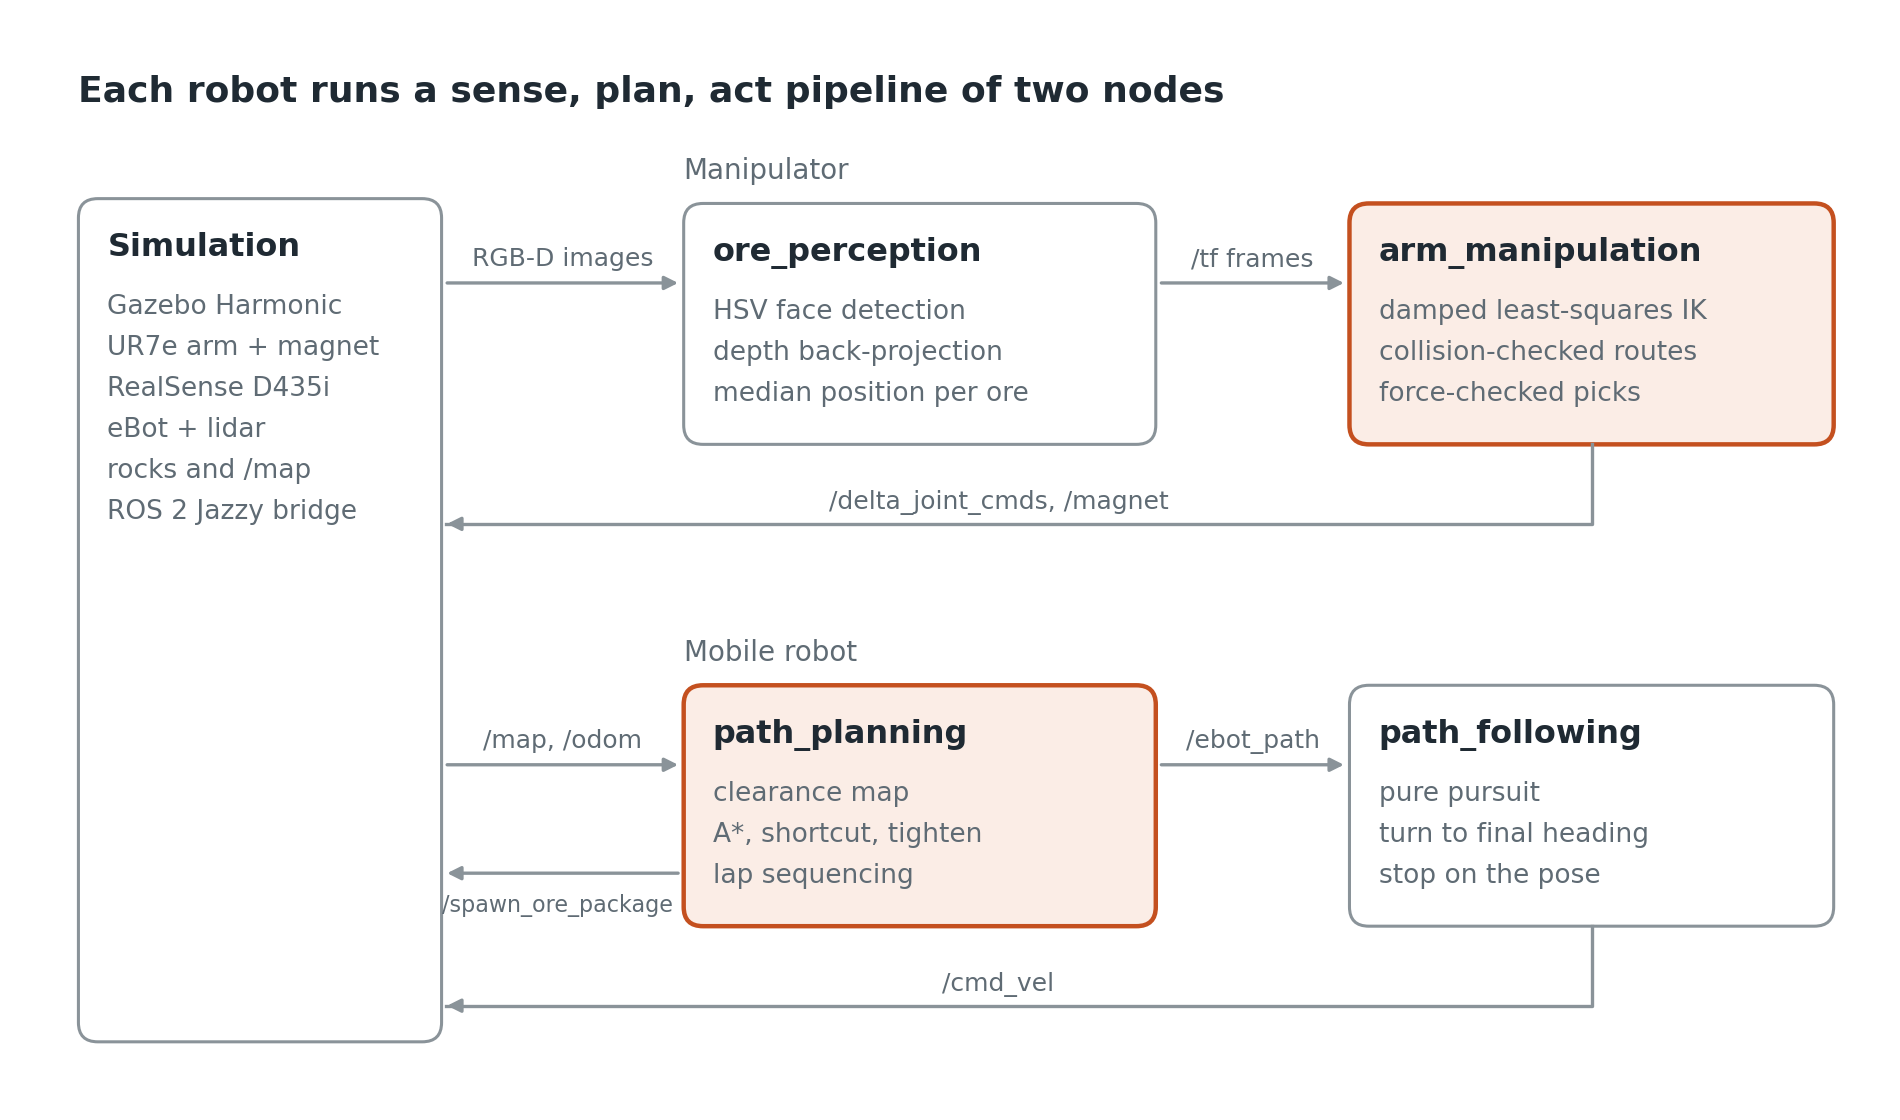
\includegraphics[width=\columnwidth]{figures/architecture.png}}
\caption{Node architecture. Feedback topics (\texttt{/tcp\_pose\_raw}, \texttt{/joint\_states}, the tool force and \texttt{/arm\_status} for the arm; \texttt{/odom} for the mobile robot) are omitted for clarity.}
\label{fig:arch}
\end{figure}

The arm is a UR7e with an electromagnet on its flange and a RealSense D435i camera fixed to its base, looking down at a conveyor. Its servo caps each joint at 0.60~rad/s and triggers a latching protective stop on joint limits, singularities, collisions and overload. The mobile robot is a skid-steer base with a 2D lidar; a static occupancy grid of the arena is published once on \texttt{/map}.

\section{Perception}
Each ore is a $101.6\times101.6\times76.2$~mm block, black except for a coloured top face. A first detector thresholded each mineral's colour tightly in HSV and kept blobs of plausible size and squareness. That works only while every ore shows one clean, saturated colour. Real ore is rarely so pure: veins of other minerals, dark or iron-stained matrix, dust and changing light all break a tight threshold. The final detector therefore separates \emph{where} an ore is from \emph{what} it is.

\subsection{Finding ores by shape}
Every pixel $(u,v)$ of the aligned depth image is back-projected with its depth $z$ through the camera intrinsics,
\begin{equation}
\mathbf{p}_c = \left(\frac{(u-c_x)z}{f_x},\ \frac{(v-c_y)z}{f_y},\ z\right), \label{eq:backproj}
\end{equation}
and transformed into the arm's \texttt{base\_link} frame. An ore's top face is the only surface on the conveyor 66--86~mm above the belt, so the pixels in that height band, split into connected regions, are the candidate faces; the band also leaves a gap between ores standing close together, where their sides would join up. A region is kept only if a rectangle fitted to its points measures 80--130~mm a side. The face centre is the centre of that rectangle: the median of the points, used at first, was pulled 4--9~mm towards the camera by edge pixels whose depth mixes with the background. Against the simulator's ground truth the centres were 1.7--2.7~mm off.

\subsection{Classifying by a colour vote}
Each face is then classified by a vote over all of its pixels. For each mineral we count the share of the face whose hue falls in that mineral's range (blue 95--130, green 40--90, orange-red 0--20 and 170--180 on OpenCV's 0--180 scale), with saturation and value floors that exclude only grey, black and white matrix ($S\ge80$; $V\ge15$ for blue, since real azurite is very dark, and $V\ge40$ for green). Orange is held to higher limits ($S\ge140$, $V\ge100$) so that brown, iron-stained rock does not count as vanadinite. The mineral with the largest share wins if it covers at least 3\% of the face and twice the share of any other colour; otherwise the face is marked \emph{uncertain}. Impurities therefore only lower the winning share instead of breaking the detection. Over the 20 frames observed before naming, faces closer than 5~cm are one ore and its mineral is the majority vote; an ore that never gets a clear vote is reported rather than guessed. Each mineral is numbered from 1, nearest the arm first, and published as a tf2 frame at 10~Hz at the median of its last 30 positions (Fig.~\ref{fig:detect}).

\begin{figure}[htbp]
\centerline{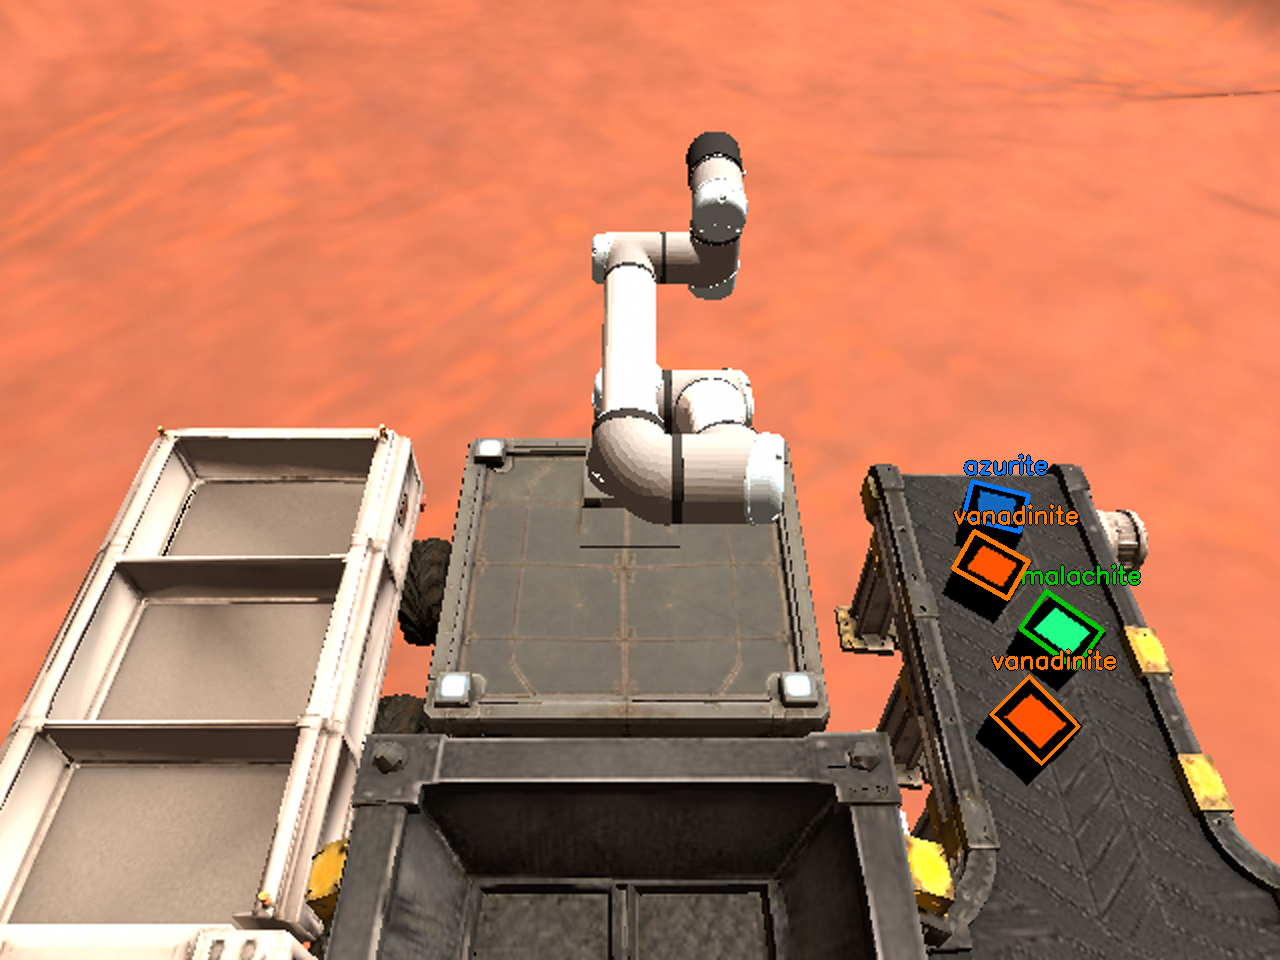
\includegraphics[width=\columnwidth]{figures/detection.png}}
\caption{RealSense colour frame with four detected ores on the conveyor (right). The cargo rover's three containers are at the left.}
\label{fig:detect}
\end{figure}

\subsection{Robustness to impure ores}
The simulated ores are pure, so impurities were painted into a captured camera frame: random blotches of dark rock (40\%), brown matrix (30\%), white quartz (15\%) and veins of the other two minerals (15\%), covering 0--70\% of each ore's coloured area, under random brightness ($\times$0.6--1.3), colour cast ($\pm$8\% per channel) and sensor noise. Fig.~\ref{fig:impurity} shows 40 trials of four ores at each level. The first detector already misses 3\% of clean ores under dim light and finds under half at 20\% impurity. The voting detector classifies every ore correctly up to 50\% impurity and 84\% at 70\%, and never assigns a wrong mineral: what it cannot decide it marks uncertain, so no ore is dropped in the wrong container.

\begin{figure}[htbp]
\centerline{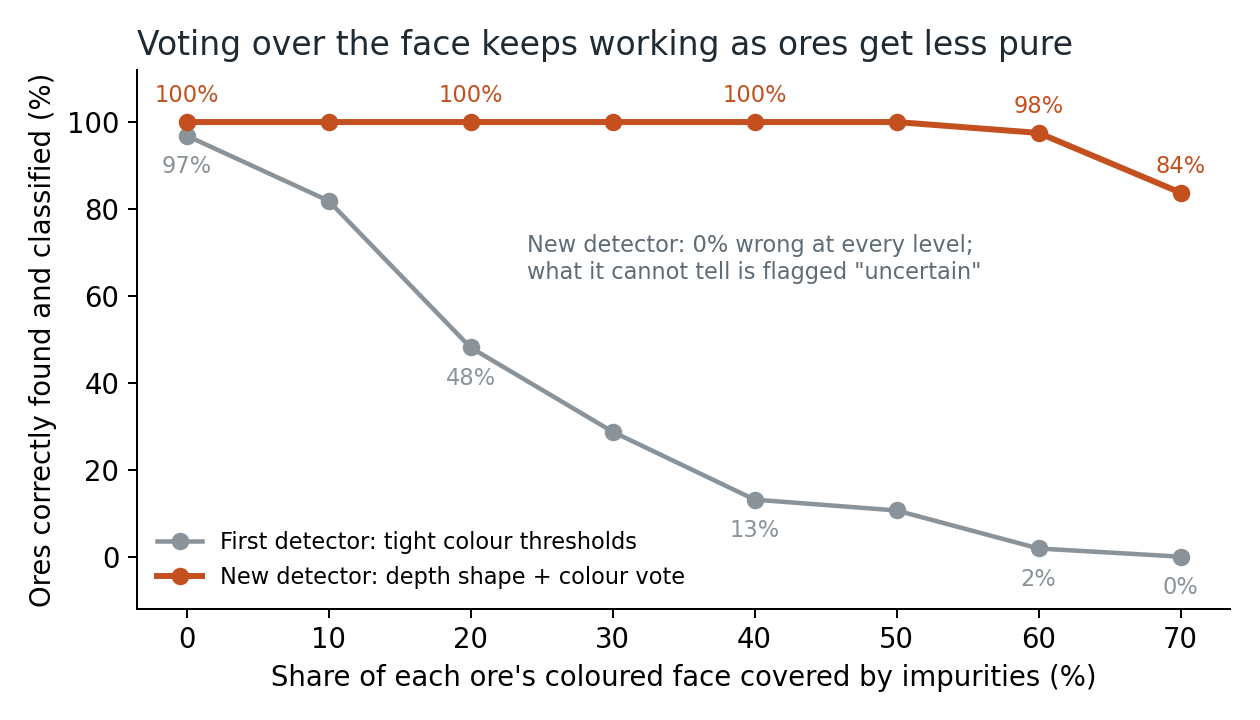
\includegraphics[width=\columnwidth]{figures/impurity.png}}
\caption{Ores correctly found and classified against the share of each ore's coloured face covered by painted impurities, 160 ores per level.}
\label{fig:impurity}
\end{figure}

\subsection{Real mineral photographs}
Painted impurities are still synthetic, so both classifiers were also run on 180 real specimen photographs from Wikimedia Commons~\cite{commons}, 60 each of azurite, malachite and vanadinite, many of them intergrown with other minerals and matrix. A photograph has no depth, so the specimen is separated from its plain backdrop by its colour distance in Lab from the median border colour. The value floors and vote limits above were chosen by a grid search on photos 1--30 of each mineral, maximising correct minus twice wrong, and are reported on the 90 held-out photos (Table~\ref{tab:photos}).

\begin{table}[htbp]
\caption{Classification of 90 Held-Out Real Photographs}
\begin{center}
\begin{tabular}{|l|c|c|c|c|}
\hline
 & \textbf{First} & \multicolumn{3}{c|}{\textbf{Voting detector}} \\
\cline{3-5}
\textbf{Mineral} & \textbf{detector} & \textbf{Correct} & \textbf{Wrong} & \textbf{Uncertain} \\
\hline
Azurite & 10\% & 37\% & 17\% & 47\% \\
\hline
Malachite & 7\% & 80\% & 7\% & 13\% \\
\hline
Vanadinite & 17\% & 93\% & 0\% & 7\% \\
\hline
\textbf{All} & \textbf{11\%} & \textbf{70\%} & \textbf{8\%} & \textbf{22\%} \\
\hline
\end{tabular}
\label{tab:photos}
\end{center}
\end{table}

The tight thresholds tuned to clean simulated faces recognise only 11\% of real specimens; the voting detector recognises 70\%. With the limits taken straight from the simulator it reached 57\% with 2\% wrong, so calibration trades a few more mistakes for many fewer uncertain specimens. Azurite remains the hardest: it is a very dark blue, and many azurite specimens are crusted with green malachite, which the two-to-one rule rightly refuses to call. A classifier trained on labelled images, such as a small convolutional network, is the natural next step once real ore samples are available.



\section{Manipulation}
\subsection{Workspace and containers}
The container positions are not given. They were extracted by parsing the cargo rover's collision mesh (a GLB file) and transforming its vertices into \texttt{base\_link}. Each container's interior spans 0.40~m in $y$ and 0.26--0.31~m in $x$. The centre of the vanadinite container lies 0.93~m from the arm base, beyond reach with the tool vertical, so each ore is released over the point of its container nearest the arm, 8~cm in from the walls (Fig.~\ref{fig:workspace}).

\begin{figure}[htbp]
\centerline{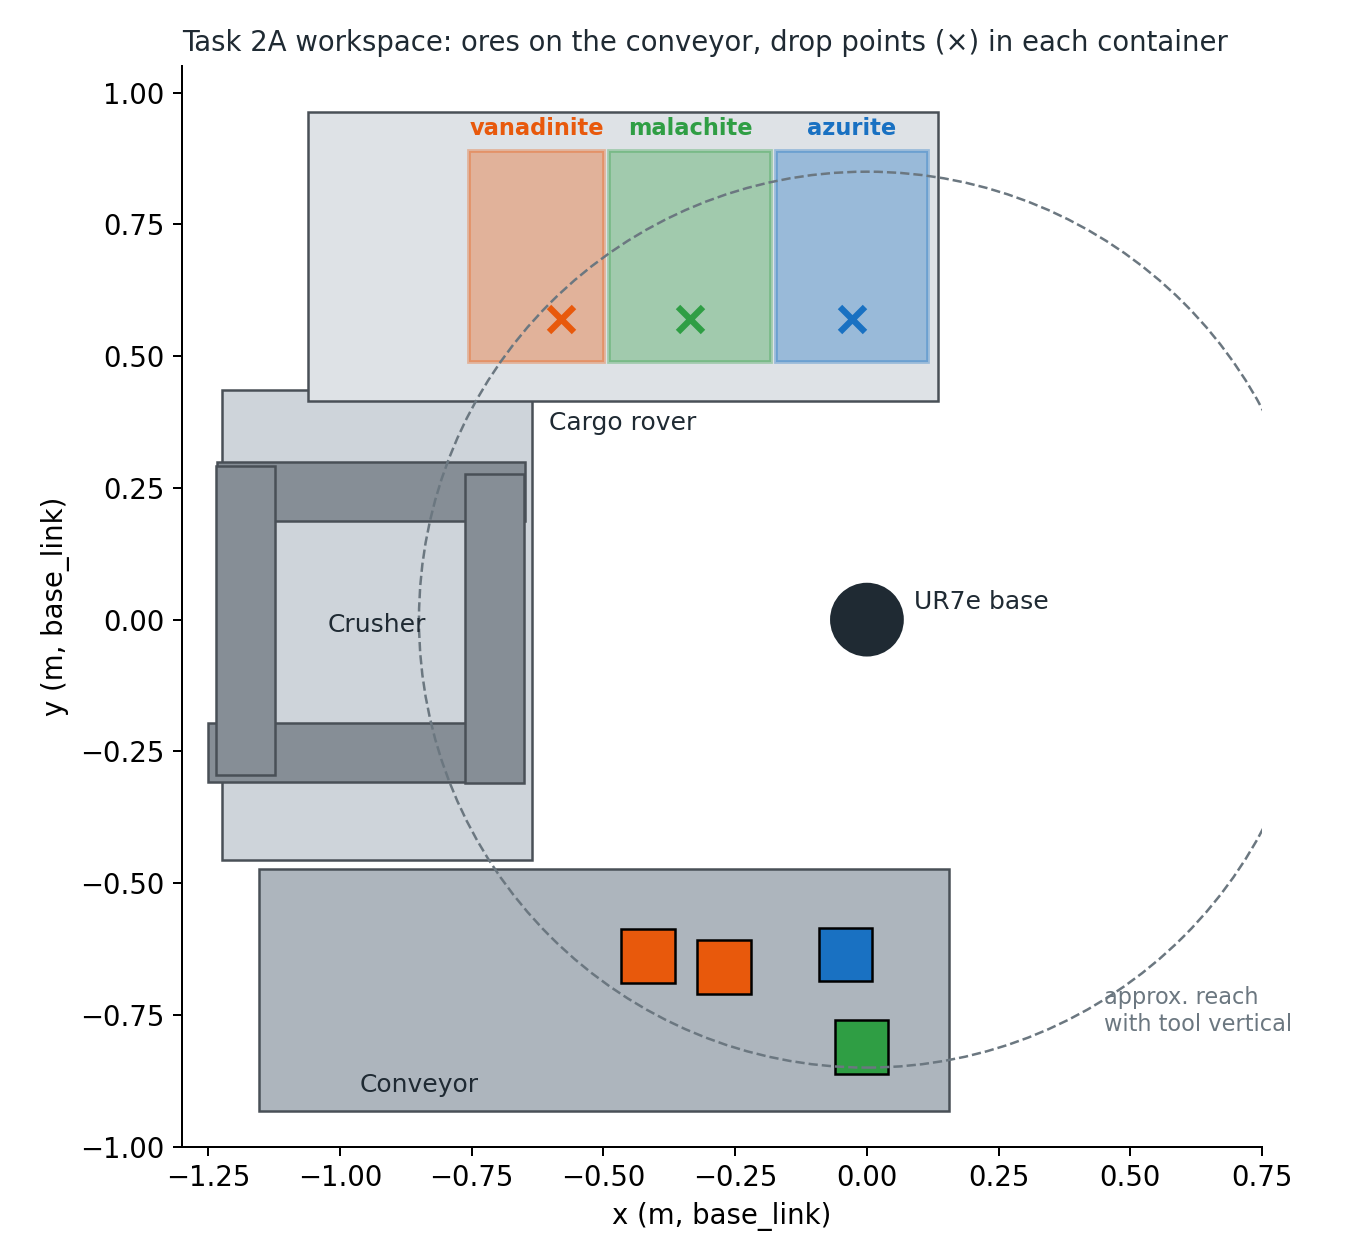
\includegraphics[width=0.92\columnwidth]{figures/workspace.png}}
\caption{Top view of the arm workspace in \texttt{base\_link}: equipment modelled as boxes for collision checking, ores on the conveyor, and the drop point ($\times$) in each container.}
\label{fig:workspace}
\end{figure}

\subsection{Inverse kinematics}
The robot model, including a point cloud of each link's collision mesh, is read from \texttt{/robot\_description}. Because the magnet face is a disc, rotation about the vertical is free, and inverse kinematics solves five constraints: the tool position $\mathbf{p}$ and a vertical tool axis $\mathbf{z}$. With error $\mathbf{e} = [\mathbf{p}^{*}-\mathbf{p};\ (\mathbf{z}\times-\hat{\mathbf{k}})_{xy}]$ and the corresponding $5\times6$ rows $J$ of the numerical Jacobian, each iteration applies the damped least-squares step~\cite{wampler1986}
\begin{equation}
\Delta\mathbf{q} = J^{T}\left(JJ^{T}+\lambda^{2}I\right)^{-1}\mathbf{e},\qquad \lambda=0.02, \label{eq:dls}
\end{equation}
clamped to 0.3~rad. A converged solution is accepted only if it lies inside the joint limits with a 0.3~rad margin, keeps the arm 3~cm from every obstacle box, keeps the tool within $1^\circ$ of vertical and keeps the smallest singular value of the Jacobian above 0.04. Each accepted configuration is stored, and the stored configurations nearest a new target are used as extra seeds. Without these seeds, IK started above the containers failed to find its way back to the conveyor. An earlier version used a constrained SLSQP optimiser and took minutes per plan; the solver of~(\ref{eq:dls}) plans in 0.1--0.4~s.

\subsection{Motion and picking}
Large moves are straight lines in joint space, accepted if the swept configurations keep 2.5~cm of clearance. Otherwise the planner tries a lift--traverse--descend detour at 0.30--0.50~m, then a route through a staging point over open floor. While an ore is carried, its block is added to the collision geometry hanging below the tool. Joint targets are tracked with a proportional controller capped at 0.30~rad/s.

The magnet face is an 81~mm disc and the ore face 101.6~mm square, so the tool must arrive within about 10~mm of the face centre and parallel to it. Vertical moves therefore use resolved-rate control~\cite{whitney1969}: a desired tool velocity $\mathbf{v}$, proportional to the position error and capped, and a tilt correction $\boldsymbol{\omega}$ are mapped to joint velocities by $\dot{\mathbf{q}} = J^{+}[\mathbf{v};\boldsymbol{\omega}]$. Each pick hovers 10~cm above the face, switches the magnet on, descends at 4~cm/s and then 1.2~cm/s, and stops at the face or when the contact force exceeds 2.5~N. After lifting, the tool force (tool weight removed) reads about 1.47~N if a 0.15~kg ore is held; below 0.8~N the pick is retried, up to three times. If a protective stop latches, the node unlocks the arm, backs off upward and re-plans the interrupted step.

\section{Path Planning and Following}
\subsection{Problem}
The mobile robot drives from home $(0,0)$ to the ore drop pose $(6.0,1.9)$, requests the ore package, continues to the arm pose $(0,1.9)$ and returns home. A path is valid if it starts and ends exactly on these poses and crosses no occupied cell; the robot must stay within 0.5~m of it and stop within 0.3~m and 0.15~rad of each pose. Path quality is measured by efficiency,
\begin{equation}
\eta = \min\!\left(1,\ \frac{L_{\text{ref}}}{L_{\text{path}}}\right), \label{eq:eff}
\end{equation}
where the reference length $L_{\text{ref}}$ is the shortest path for a 0.395~m circle enclosing the $0.62\times0.49$~m chassis.

\subsection{Planner}
A Euclidean distance transform of the 5~mm \texttt{/map} ($1784\times1380$ cells) gives every cell its clearance to the nearest rock or wall. A 5~cm grid sampled at cell centres is searched by 8-connected A*~\cite{hart1968} over the cells whose clearance meets a chosen level $c$. Near the fixed start and end poses the limit drops to 0.30~m, since the ore drop pose lies only 0.375~m from the arena wall. The A* route is then shortcut, joining each point to the furthest later point visible with clearance $c$, and tightened: each corner is pulled towards the chord between its neighbours, halving the step until both legs still clear. Every straight leg is verified on the full-resolution map at 5~mm spacing. Tightening removes the grid's quantisation, so the path wraps each rock at exactly the clearance asked for (Fig.~\ref{fig:paths}).

\begin{figure}[htbp]
\centerline{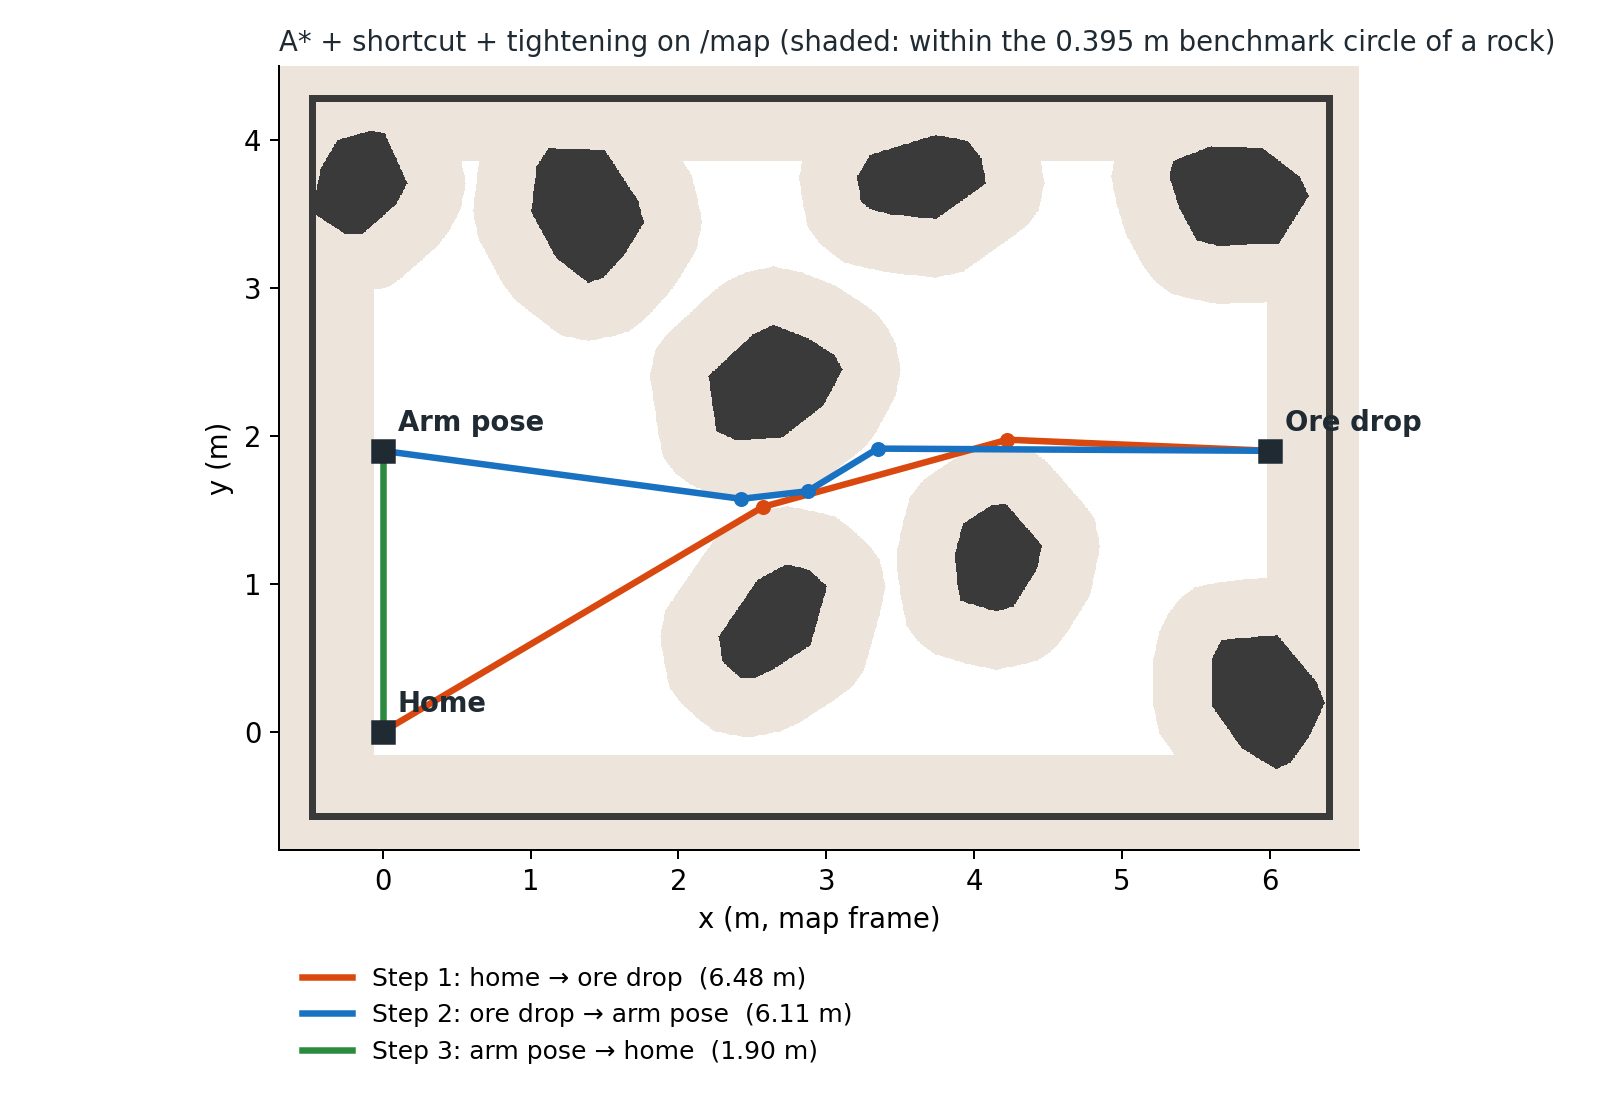
\includegraphics[width=\columnwidth]{figures/paths.png}}
\caption{Planned paths for the three legs of the lap. Shaded cells lie within 0.395~m of a rock or wall.}
\label{fig:paths}
\end{figure}

\subsection{Choosing the clearance}
The reference path treats the robot as a 0.395~m circle, but when driving straight past a rock only its 0.245~m half-width must clear. Fig.~\ref{fig:tradeoff} shows the trade-off on one rock layout: below about 0.40~m the lap length is nearly flat, while above it narrow gaps close and the lap grows by up to 13\%. The planner first plans at 0.395~m to estimate the reference path, then tries levels from 0.40 down to 0.34~m and selects the safest whose length is within 1~cm of that estimate. At 0.38~m the robot keeps 13.5~cm to each side, against a measured tracking error of at most 9~cm.

\begin{figure}[htbp]
\centerline{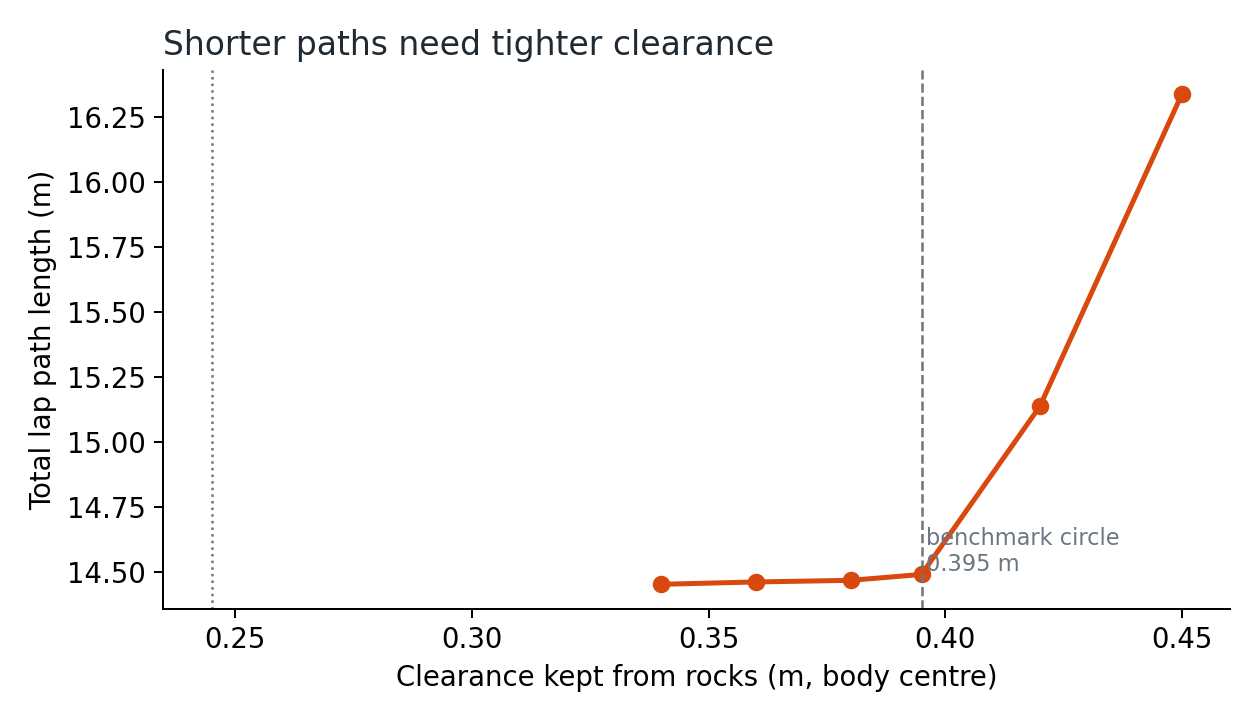
\includegraphics[width=0.92\columnwidth]{figures/tradeoff.png}}
\caption{Total lap length against the clearance kept from rocks, for one rock layout. No path exists above 0.45~m.}
\label{fig:tradeoff}
\end{figure}

\subsection{Follower}
The follower is a pure-pursuit controller~\cite{coulter1992} with a 0.30~m lookahead and a 0.35~m/s cruise speed. It turns on the spot when the heading error exceeds $40^\circ$, slows on the approach to the end of the path, then turns to the path's final heading and stops. It drives the published path without re-planning; the lidar only slows it near obstacles. The planner watches \texttt{/odom}, advances to the next leg after the robot has stood still on the end pose for 0.5~s, and at the ore drop pose calls \texttt{/spawn\_ore\_package} asynchronously.

\section{Integration: Hand-off and Re-planning}
\subsection{Hand-off from the mobile robot to the arm}
To run the whole loop, the arm is spawned into the mobile robot's world. In hand-off mode the planner stops after the second leg, at the arm pose, publishes \texttt{/handoff/ready} and waits. A hand-off node, built on the same arm model, planner and controllers as the sorting node, then takes over. It locates the ore package from the eBot's odometry (which matches the simulator's ground truth to the millimetre), refines its height and, when the whole face is in view, its centre from the depth camera; in testing it was within 4~mm of the truth. The eBot's body is added to the arm's collision boxes. The package ($177.8\times139.7\times76.2$~mm, 0.30~kg) is picked with the magnet and confirmed by the force sensor at 2.94~N, lifted straight up until it clears the deck by 7~cm, carried with its block in the collision model, lowered onto the conveyor intake and released. The node then publishes \texttt{/handoff/done} and the eBot drives home. A full mission takes about 2~minutes.

\subsection{Re-planning around unmapped obstacles}
Every planned path keeps at least 0.30~m from the rocks on \texttt{/map}, so a lidar return within 0.26~m of the next 1.6~m of path cannot be a mapped rock; it is also where the 0.245~m half-width chassis would hit it. After three consecutive sightings the follower stops and publishes the lidar points around the robot on \texttt{/ebot\_obstacles}. The planner marks them as occupied, recomputes the distance transform and plans a new path from where the robot stands, in about 0.1~s. In a test where a box was dropped on the path mid-leg, the robot stopped, followed the new path and completed the lap, never coming closer than 1.16~m to the box's centre.

\section{Results}
Each trial used a freshly launched world with randomised ore positions or rock layout, and was assessed by the automated evaluator supplied with the simulation. Table~\ref{tab:results} summarises the trials.

\begin{table}[htbp]
\caption{Trial Results}
\begin{center}
\begin{tabular}{|c|p{6.4cm}|}
\hline
\textbf{Trial} & \textbf{Outcome} \\
\hline
Arm 1 & 4/4 ores detected, picked and dropped in the correct container; 0 safety stops \\
\hline
Arm 2 & Different ore mix, one ore 0.83~m from the base: 4/4 sorted correctly in 167~s; 0 safety stops \\
\hline
Arm 3 & Voting detector (simulator limits): 4/4 classified in 20/20 frames, sorted correctly; 0 safety stops \\
\hline
Arm 4 & Voting detector (calibrated limits), two azurite ores: 4/4 sorted correctly in 180~s; 0 safety stops \\
\hline
Robot 1 & First planner: 14.74~m lap vs.\ 14.46~m reference, $\eta=0.98$ \\
\hline
Robot 2 & Final planner: 14.55~m vs.\ 14.58~m, $\eta=1.00$ \\
\hline
Robot 3 & Final planner: 14.48~m vs.\ 14.43~m, $\eta=0.996$ \\
\hline
\end{tabular}
\label{tab:results}
\end{center}
\end{table}

All robot trials collected the ore package without a collision, kept the robot within 0.09~m of its paths and stopped within 0.15~m and 0.04~rad of each pose. Every pick was confirmed at 1.46--1.47~N. The small shortfall in trial Robot~3 comes from the reference itself: on the same rock layout the reference length of the second leg measured 6.14~m in one trial and 6.07~m in the next, while the planned path stayed at 6.11~m. Closing that gap reliably would require clearances below 0.34~m, at a real risk of collision.

\section{Challenges and Lessons}
Table~\ref{tab:issues} summarises the main problems found during testing. Most were invisible until the robots were run end to end and assessed automatically.

\begin{table}[htbp]
\caption{Main Problems and Fixes}
\begin{center}
\begin{tabular}{|p{2.3cm}|p{5.4cm}|}
\hline
\textbf{Problem} & \textbf{Cause and fix} \\
\hline
No path found & Drop pose 0.375~m from the wall, plus clearance lost to map downsampling. Fixed by full-resolution clearance and a relaxed limit near fixed poses. \\
\hline
Paths 2\% long & Coarse-grid checks and grid-snapped corners. Fixed by fine-map checks, tightening and reference-aware clearance. \\
\hline
IK slow or stuck & SLSQP evaluated all checks in every gradient step; poor seeds over the containers. Fixed by DLS IK and a seed library. \\
\hline
Vanadinite unreachable & Container centre 0.93~m away. Fixed by releasing at the nearest reachable point inside it. \\
\hline
Ores never found & tf frame list writes a space after each name. Fixed by a regular-expression parse. \\
\hline
\end{tabular}
\label{tab:issues}
\end{center}
\end{table}

Three lessons stand out. Testing end to end against an automatic evaluator early exposed losses that plots did not. Measuring the geometry ourselves revealed both the wall beside the drop pose and the unreachable container centre. And a solver specific to the problem, with checks applied once to its result, was about 300 times faster than a general constrained optimiser.

\section{Conclusion}
Both robots complete their missions end to end in simulation, using only planners and controllers written for this project: every ore was sorted correctly and every lap was completed without a collision. The two robots also work together: the mobile robot hands the ore package to the arm, and re-plans around obstacles the map does not contain. Future work includes a classifier trained on real ore samples, faster sorting by blending moves and ordering picks, and a move to physical hardware, where lighting and sensor noise will test the colour thresholds and the force-based pick check.

\section*{Acknowledgment}
We thank e-Yantra, IIT Bombay, for the Strata Cobot simulation environment and its evaluation tools.

\begin{thebibliography}{00}
\bibitem{eyantra} e-Yantra, IIT Bombay, ``Strata Cobot (SC) theme,'' e-Yantra Robotics Competition 2026--27 portal. [Online]. Available: \url{https://portal.e-yantra.org/courses/theme_sc/}
\bibitem{hart1968} P. E. Hart, N. J. Nilsson, and B. Raphael, ``A formal basis for the heuristic determination of minimum cost paths,'' IEEE Trans. Syst. Sci. Cybern., vol. 4, no. 2, pp. 100--107, 1968.
\bibitem{coulter1992} R. C. Coulter, ``Implementation of the pure pursuit path tracking algorithm,'' Carnegie Mellon Univ., Pittsburgh, PA, USA, Tech. Rep. CMU-RI-TR-92-01, 1992.
\bibitem{wampler1986} C. W. Wampler, ``Manipulator inverse kinematic solutions based on vector formulations and damped least-squares methods,'' IEEE Trans. Syst., Man, Cybern., vol. 16, no. 1, pp. 93--101, 1986.
\bibitem{whitney1969} D. E. Whitney, ``Resolved motion rate control of manipulators and human prostheses,'' IEEE Trans. Man-Mach. Syst., vol. 10, no. 2, pp. 47--53, 1969.
\bibitem{commons} Wikimedia Commons, ``Category:Azurite'', ``Category:Malachite'' and ``Category:Vanadinite,'' accessed Oct.\ 2026. [Online]. Available: \url{https://commons.wikimedia.org/wiki/Category:Minerals}
\bibitem{macenski2022} S. Macenski, T. Foote, B. Gerkey, C. Lalancette, and W. Woodall, ``Robot Operating System 2: Design, architecture, and uses in the wild,'' Sci. Robot., vol. 7, no. 66, 2022.
\end{thebibliography}

\end{document}
